\documentclass[openany,a4paper,12pt]{book}
\usepackage{graphicx}
\usepackage{amsmath}
\usepackage{amssymb}
\usepackage{bbding}
\usepackage{float}
\restylefloat{table}
\usepackage{multirow}
%\setlength{\textwidth}{+11cm}
\title{The Triangulation of Titling Data in Non-Linear Gaussian Fashion via $\rho$ Series}
\date{October 31, 2014}
\author{John Doe\\ Magic Department, Richard Miles University \and Richard Row, \LaTeX\ Academy}
\begin{document}
\bibliographystyle{plain}
\maketitle
\tableofcontents
\chapter{The Platonic Solids}
\begin{quotation}"A platonic solid is a polyhedron all of whose faces are congruent regular polygons, and where the same number of faces meet at every vertex. The best know example is a cube whose faces are six congruent squares." - John Kaiser
\end{quotation}
\begin{quotation}"Mathematics as an expression of the human mind reflects the active will, the contemplative reason, and the desire for aesthetic perfection. Its basic elements are logic and intuition, analysis and construction, generality and individuality." - Richard Courant
\end{quotation}
\begin{quotation}"For scholars and laymen alike it is not philosophy but active experience in mathematics itself that can alone answer the question: What is mathematics?" - Richard Courant
\end{quotation}
\newpage
\section{There are only five!}
The Greeks recognized that there are only five platonic solids. But why is this so? The key observation is that the interior angles of the polygons meeting at a vertex of a polyhedron add to less than 360 degrees. To see this note that if such polygons met in a plane, the interior angles of all the polygons meeting at a vertex would add to exactly 360 degrees. Now cut an angle out of paper, and fold another piece of paper to that angle along a line \cite{smith96:2}. The first piece will fit into the second piece when it is perpendicular to the fold. Think of the fold as a line coming out of our polyhedron. The faces of the polyhedron meet at the fold at angles less than 90 degrees. How can this be possible? Try wiggling your first piece of paper within the second. To be able to incline it with respect to the fold you have to decrease the angle of the first piece, or increase the angle of the second. Next we'll consider all possibilities for the number of faces meeting at a vertex of a regular polyhedron.  \\\\
For each possibility we actually construct such a polyhedron, a picture of which you can see close by on this page. Here are the possibilities: 
\begin{itemize}
\item
\textbf{Triangles}. The interior angle of an equilateral triangle is 60 degrees. Thus on a regular polyhedron, only 3, 4, or 5 triangles can meet a vertex. If there were more than 6 their angles would add up to at least 360 degrees which they can't. Consider the possibilities: 
\item
\textbf{Squares}. Since the interior angle of a square is 90 degrees, at most three squares can meet at a vertex. This is indeed possible and it gives rise to a \textbf{hexahedron} or \textbf{cube}.
\begin{itemize}
\item[\Checkmark]
\textit{3 triangles} meet at each vertex. This gives rise to a \textbf{Tetrahedron}.
\item[\Checkmark]
\textit{4 triangles} meet at each vertex. This gives rise to an \textbf{Octahedron}.
\item[\Checkmark]
\textit{5 triangles} meet at each vertex. This gives rise to an \textbf{Icosahedron}.
\end{itemize}
\item
 \textbf{Pentagons}. As in the case of cubes, the only possibility is that three pentagons meet at a vertex. This gives rise to a Dodecahedron.
\item
 \textbf{Hexagons} or regular polygons with more than six sides cannot form the faces of a regular polyhedron since their interior angles are at least 120 degrees.
 \end{itemize}
\newpage
Before continuing, let us collect some data. Let
\begin{itemize}
\item[-]
\textit{m} be the number of polygons meeting at a vertex,
\item[-]
\textit{n} the number of vertices of each polygon,
\item[-]
\textit{f} the number of faces of the polyhedron,
\item[-]
\textit{e} the number of edges of the polyhedron, and
\item[-]
\textit{v} the number of vertices of the polyhedron.
\end{itemize}

\begin{table}[H]
\begin{center}
\caption{Pair of numbers} 
\begin{tabular}{|p{2.5cm}|p{1cm}|p{1cm}|p{1cm}|p{1cm}|p{1cm}|}
\hline
    name & n & m & f & e & v \\ \hline
    Tetrahedron & 3 & 3 & 4 & 6 & 4  \\
    Octahedron & 3 & 4 & 8 & 12 & 6\\
    Icosahedron & 3 & 5 & 20 & 2 & 1 \\
    Hexahedron & 4 & 3& 6 & 9 & 4 \\
    Dodecahedron & 5 & 3 & 4 & 15 & 9 \\ \hline
\end{tabular}
\end{center}
\end{table}

Our aim now is to show that for any pair of number n and m the values of the other parameters, f, e, and v are determined uniquely. First we note that since two faces meet in one edge, we must have: 
\begin {equation}
e=\frac{nf}{2}
\end {equation}
Next, since every vertex is shared by m faces, we must have: 
\begin {equation}
v=\frac{nf}{m}
\end {equation}
It is apparent from the Table that for all five regular polyhedra
\begin {equation}
f=2+e-v
\end {equation}
We'll see below that this equations actually holds for all convex polyhedra. Given m and n the above three equations determine f, e, and v uniquely, and so there are only five possible regular polyhedra.
\newpage
\section{Euler's Polyhedron Theorem}
To see why it is true we proceed in several steps. First we remove one face from the polyhedron. Let
\begin {equation}
F=f-1
\end {equation}
be the new number of faces. We need to show
\begin {equation}
f=1+e-v
\end {equation}
Now think of the remaining faces of the polyhedron as made of rubber and stretched out on a table. This will certainly change the shape of the polygons and the angles involved, but it will not alter the number of vertices, edges, and faces. Now we draw diagonals in the stretched faces out of the Polygons. Every diagonal increase the number e of edges by one, and also the number F of faces, so that our equation \textbf{(1.5)} remains valid. We continue this process until all polygons have been changed into triangles. \newline \newline
In the final stage we remove triangles until we are left with only one triangle for which (*) is obviously true. How do we do that? If the removed triangle has exactly one edge on the boundary then F and e are both decreased by 1 and \textbf{(1.5)} remains true. If it has two edges on the boundary then F is reduced by 1, e is reduced by 2, and v is reduced by 1, so that \textbf{(1.5)} remains true.
\begin{center}

\begin{figure}[ht]
\begin{center}
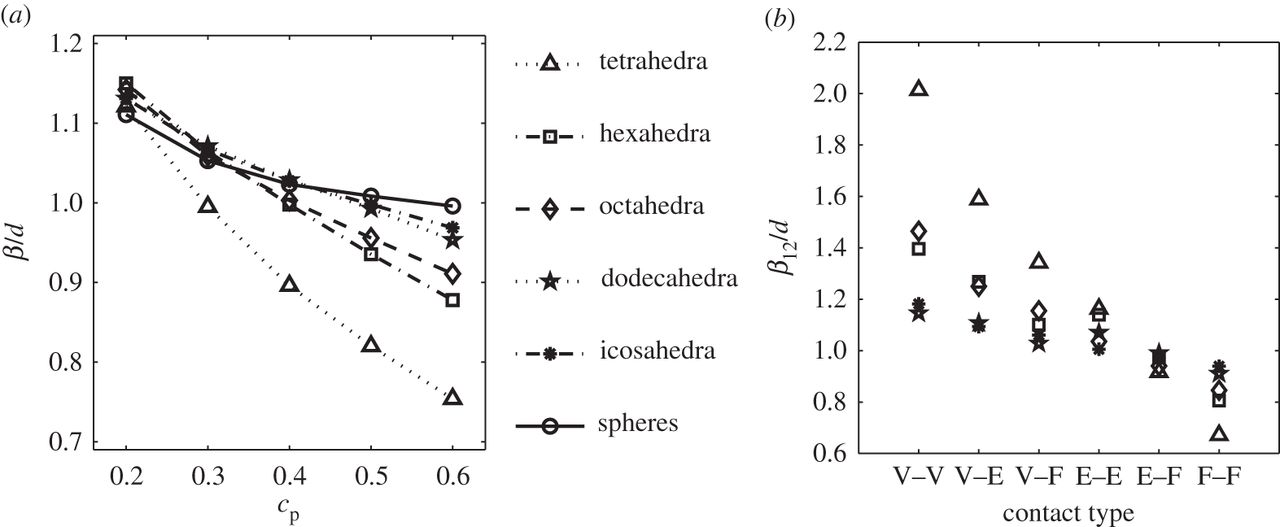
\includegraphics[width=13cm]{picture1.jpg} \caption{6 models of thermodynamics}{Third-order thermo-mechanical properties for packs of Platonic solids using statistical micromechanics} \label{rys1}
\end{center}
\end{figure}
\end{center}
\chapter{Analysis of Algorithms}
\begin{quotation}"By understanding a machine-oriented language, the programmer will tend to use a much more efficient method; it is much closer to reality..." - Donald Knuth
\end{quotation}
\begin{quotation}"I took a computer-science course to fill a prerequisite at Stanford, and I realized that every day was a new problem, and every day you got to think about how to solve something new, how to reason through something new, how to develop an algorithm to solve for something you hadn't worked on before." - Marissa Mayer
\end{quotation}
\begin{quotation}
Despite all of our technological advances, content creation still requires time, inspiration, and a certain amount of sweat. There aren't any shortcuts. You can't write an algorithm for it. You can't predict it. You can't code it. - Shawn Amos
\end{quotation}

\newpage
\section{Cost models}
Time efficiency estimates depend on what we define to be a step. For the analysis to correspond usefully to the actual execution time, the time required to perform a step must be guaranteed to be bounded above by a constant. One must be careful here; for instance, some analyses count an addition of two numbers as one step. This assumption may not be warranted in certain contexts. For example, if the numbers involved in a computation may be arbitrarily large, the time required by a single addition can no longer be assumed to be constant.
\newline \newline
Two cost models are generally used:
\begin{enumerate}
\item 
the uniform cost model, also called uniform-cost measurement (and similar variations), assigns a constant cost to every machine operation, regardless of the size of the numbers involved
\item
the logarithmic cost model, also called logarithmic-cost measurement (and similar variations), assigns a cost to every machine operation proportional to the number of bits involved \cite{Abedon94:5}
\end{enumerate}
\begin{center}

\begin{figure}[ht]
\begin{center}
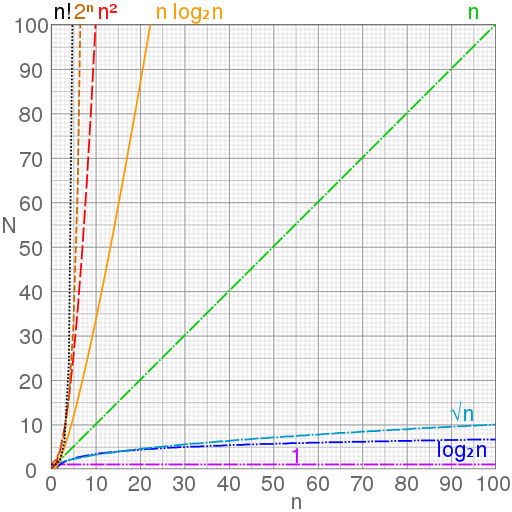
\includegraphics[width=8cm]{picture2.png} \caption{Graph of number of operations}{The analysis of algorithms, N vs input size, n for common complexities, assuming a coefficient of 1} \label{rys2}
\end{center}
\end{figure}
\end{center}
Run-time analysis is a theoretical classification that estimates and anticipates the increase in running time (or run-time) of an algorithm as its input size (usually denoted as n) increases. Run-time efficiency is a topic of great interest in computer science: A program can take seconds, hours or even years to finish executing, depending on which algorithm it implements (see also performance analysis, which is the analysis of an algorithm's run-time in practice).\cite{goossens93:3}
\section{Shortcomings of empirical metrics}

Since algorithms are platform-independent (i.e. a given algorithm can be implemented in an arbitrary programming language on an arbitrary computer running an arbitrary operating system), there are significant drawbacks to using an empirical approach to gauge the comparative performance of a given set of algorithms.
\newline\\
Take as an example a program that looks up a specific entry in a sorted list of size n. Suppose this program were implemented on Computer A, a state-of-the-art machine, using a linear search algorithm, and on Computer B, a much slower machine, using a binary search algorithm.

\begin{table}[H]
\caption{I/O - input/output algorithm} 
\begin{center} 
\begin{tabular}{|c|c|c|}
\hline \ $q1/q2$ & 0 & 1 \\ \hline
0 & $\frac{d{v} c}{d t} = -\frac{1}{C}I_{load}$ & $\frac{L{i} c}{d t} = \frac{63}{V}I_{i}$  \\
1 & $\frac{d{v} c}{d t} = -\frac{R_{l}}{L} i_{L}- \frac{1}{C}I_{load}$ & $\frac{R{i} V}{d t} = -\frac{R_{i}}{V} i_{L}- \frac{1}{V}I_{load}$ \\ \hline
\end{tabular}
\end{center}
\end{table}
\section{Evaluating run-time complexity}
As a rule-of-thumb \cite{greenwade93:1}, one can assume that the highest-order term in any given function dominates its rate of growth and thus defines its run-time order. In this example, $n^2$ is the highest-order term, so one can conclude that $f(n) = O(n^2)$. Formally this can be proven as follows:
\begin{equation}
\bigg[\frac{1}{2}(n^2+n)\bigg]T_{6}+\bigg[\frac{1}{2}(n^2+3n)\bigg]T_{5}+(n+1)T_{4}+T_{1}+T_{2}+T_{3}+T_{7}<cn^2, n \geq n_{0}
\end{equation}
\begin{table}[H]
\caption{Platform-independent algorithms} 
\begin{center} 
\begin{tabular}{|l|p{3cm}|p{3cm}|}
\hline \textbf{n} & \textbf{Computer A run-time (in nanoseconds)} & \textbf{Computer B run-time (in nanoseconds)} \\ \hline
16 & 8 & 100,000 \\
63 & 32 & 150,000 \\
250 & 125 & 200,000 \\
1,000 & 500 & 250,000 \\ \hline
\end{tabular}
\end{center}
\end{table}
$$\sin (2x)=\frac{2\cos (x)+\frac{sin (x)}{cos (x)}}{1-\tan^2(x)}$$
\begin{multline*}
p(x) = 3x^6 + 14x^5y + 590x^4y^2 + 19x^3y^3\\ 
- 12x^2y^4 - 12xy^5 + 2y^6 - a^3b^3
\end{multline*}
\begin{align*} 
2x - 5y &=  8 \\ 
3x + 9y &=  -12
\end{align*}
\begin{align*}
x&=y           &  w &=z              &  a&=b+c\\
2x&=-y         &  3w&=\frac{1}{2}z   &  a&=b\\
-4 + 5x&=2+y   &  w+2&=-1+w          &  ab&=cb
\end{align*}
Suppose this program were implemented on Computer A, a state-of-the-art machine, using a linear search algorithm:

\begin{equation}
\lim_{n \to \infty} a_{n} = g \Leftrightarrow
\forall {\varepsilon > 0} \;
\forall {n > N_{\varepsilon}} \colon
\left| {a_{n} - g} \right| < \varepsilon
\end{equation}
\[ \sum_{i=1}^{\infty} \frac{1}{n^s} 
= \prod_p \frac{1}{1 - p^{-s}} \]

\begin{gather*}
a_0=\frac{1}{\pi}\int\limits_{-\pi}^{\pi}f(x)\,\mathrm{d}x\\[6pt]
\begin{split}
a_n=\frac{1}{\pi}\int\limits_{-\pi}^{\pi}f(x)\cos nx\,\mathrm{d}x=\\
=\frac{1}{\pi}\int\limits_{-\pi}^{\pi}x^2\cos nx\,\mathrm{d}x
\end{split}\\[6pt]
\begin{split}
b_n=\frac{1}{\pi}\int\limits_{-\pi}^{\pi}f(x)\sin nx\,\mathrm{d}x=\\
=\frac{1}{\pi}\int\limits_{-\pi}^{\pi}x^2\sin nx\,\mathrm{d}x
\end{split}\\[6pt]
\end{gather*}
\begin{equation}
  x = a_0 + \frac{1}{\displaystyle a_1 
          + \frac{1}{\displaystyle a_2 
          + \frac{1}{\displaystyle a_3 + a_4}}}
\end{equation}
\begin{table}[H]
\caption{Powers of prime numbers} 
\begin{center} 

\begin{tabular}{cc|c|c|c|c|l}

\cline{3-6}
& & \multicolumn{4}{ c| }{Primes} \\ \cline{3-6}
& & $x_{0}+x_{-1}+x_{-2}$ & 3 & 5 & 7 \\ \cline{1-6}
\multicolumn{1}{ |c  }{\multirow{2}{*}{Powers} } &
\multicolumn{1}{ |c| }{$\frac{1}{9}$} &$2x^4+4x^3+2x^2+\dfrac{(x+2)(x+4)}{4}$ & $\frac{1}{3}$ & $\frac{1}{16}$ & $\frac{1}{32}$ &     \\ \cline{2-6}
\multicolumn{1}{ |c  }{}                        &
\multicolumn{1}{ |c| }{540} & $3x^5+4x^4+5x^2+(x+2)(x+4)$ & $\frac{1}{256}$ & $\frac{1}{512}$ & $\frac{1}{1024}$ &     \\ \cline{1-6}
\multicolumn{1}{ |c  }{\multirow{2}{*}{Powers} } &
\multicolumn{1}{ |c| }{gcd} & $2x^4+4x^3+2x^2+(x+2)(x+4)$ & 2 & 0 & 0 & $\geq$ minimum capacity \\ \cline{2-6}
\multicolumn{1}{ |c  }{}                        &
\multicolumn{1}{ |c| }{fog} & $\sqrt{\frac{x^2}{2}}$ & $\sqrt{\frac{x^2}{4}}$ & $\sqrt{\frac{x^2}{8}}$ & $\sqrt{\frac{x^2}{16}}$ & $\leq$ maximum capacity \\ \cline{1-6}
\end{tabular}

\end{center}
\end{table}

http://www.math.utah.edu/~pa/math/polyhedra/polyhedra.html
\chapter{The Final Frontier}
This is the final chapter
\begin{quotation}
"Space: \cite{greenwade93:1} the final frontier. These are the voyages of the starship Enterprise. Its five-year mission: to explore strange new worlds, to seek out new life and new civilizations, to boldly go where no man has gone before." \cite{AbedonHymanThomas03:4}
\end{quotation}
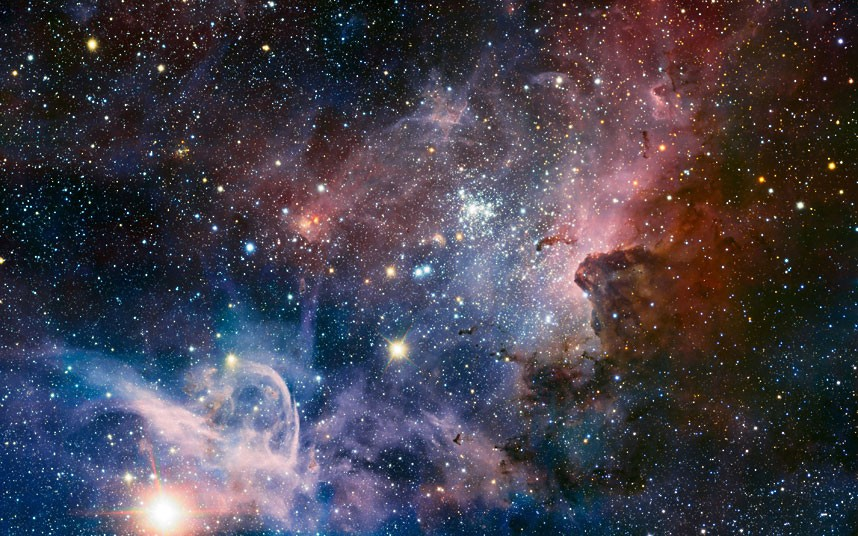
\includegraphics[angle=90,scale=0.3]{picture3.jpg}
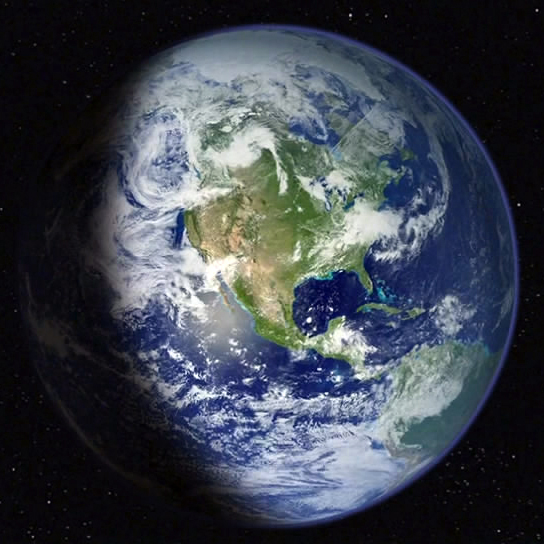
\includegraphics[angle=90,scale=0.3]{picture4.jpg}
$$ax^2+bx+c+\dfrac{12}{x+1}$$
\listoftables
\listoffigures
\bibliography{Projekt}
\end{document}
